\section{Calibration}
This section focuses on the calibration of the Rasperry Pi Camera Module V2 (resolution set to $3280\times 2464$\,pixels),
but all insights learned from these first attempts are applicable to the similar (but higher quality) cameras, which where later also used.

To capture the whole steel-spring, the camera has to be mounted approximately 250\,mm away from it.
From this distance, one pixel-width corresponds to a length within the tenths of a millimeter range.
It is therefore absolutely necessary to calibrate the camera as described in section \ref{theory:calibration}, since non-linear distortions can distort the image by 10-20\, pixels or even more.
Lens imperfections can therefore cause deviations in the measurement of several millimeters, which is not acceptable.

To calibrate a camera in OpenCV, one has to take images of a known 2D-pattern.
It is reasonable to use a checkerboard, since OpenCV provides functions to detect checkerboard-corners reliably with subpixel precision.

\subsection{How to obtain a usable calibration}
First attempts to calibrate the camera failed.
Despite reprojection errors of $<0.3$ pixels, the obtained distortion coefficients did not seem to deliver a good undistortion of the image.
Furthermore, new attempts with slightly different images of the checkerboard resulted in totally different coefficients.

It is therefore important to take a closer look at the technical aspects of the calibration process.

\subsubsection{Calibration statistics}
To get more insight what went wrong, some sort of statistics is needed.
200 images of the checkerboard from different view-points and angles has been taken.
A couple of these images are shown in Figure  \ref{development:im}

\begin{figure}[ht]
	\centering
	\subfigure[\label{development:im0}]{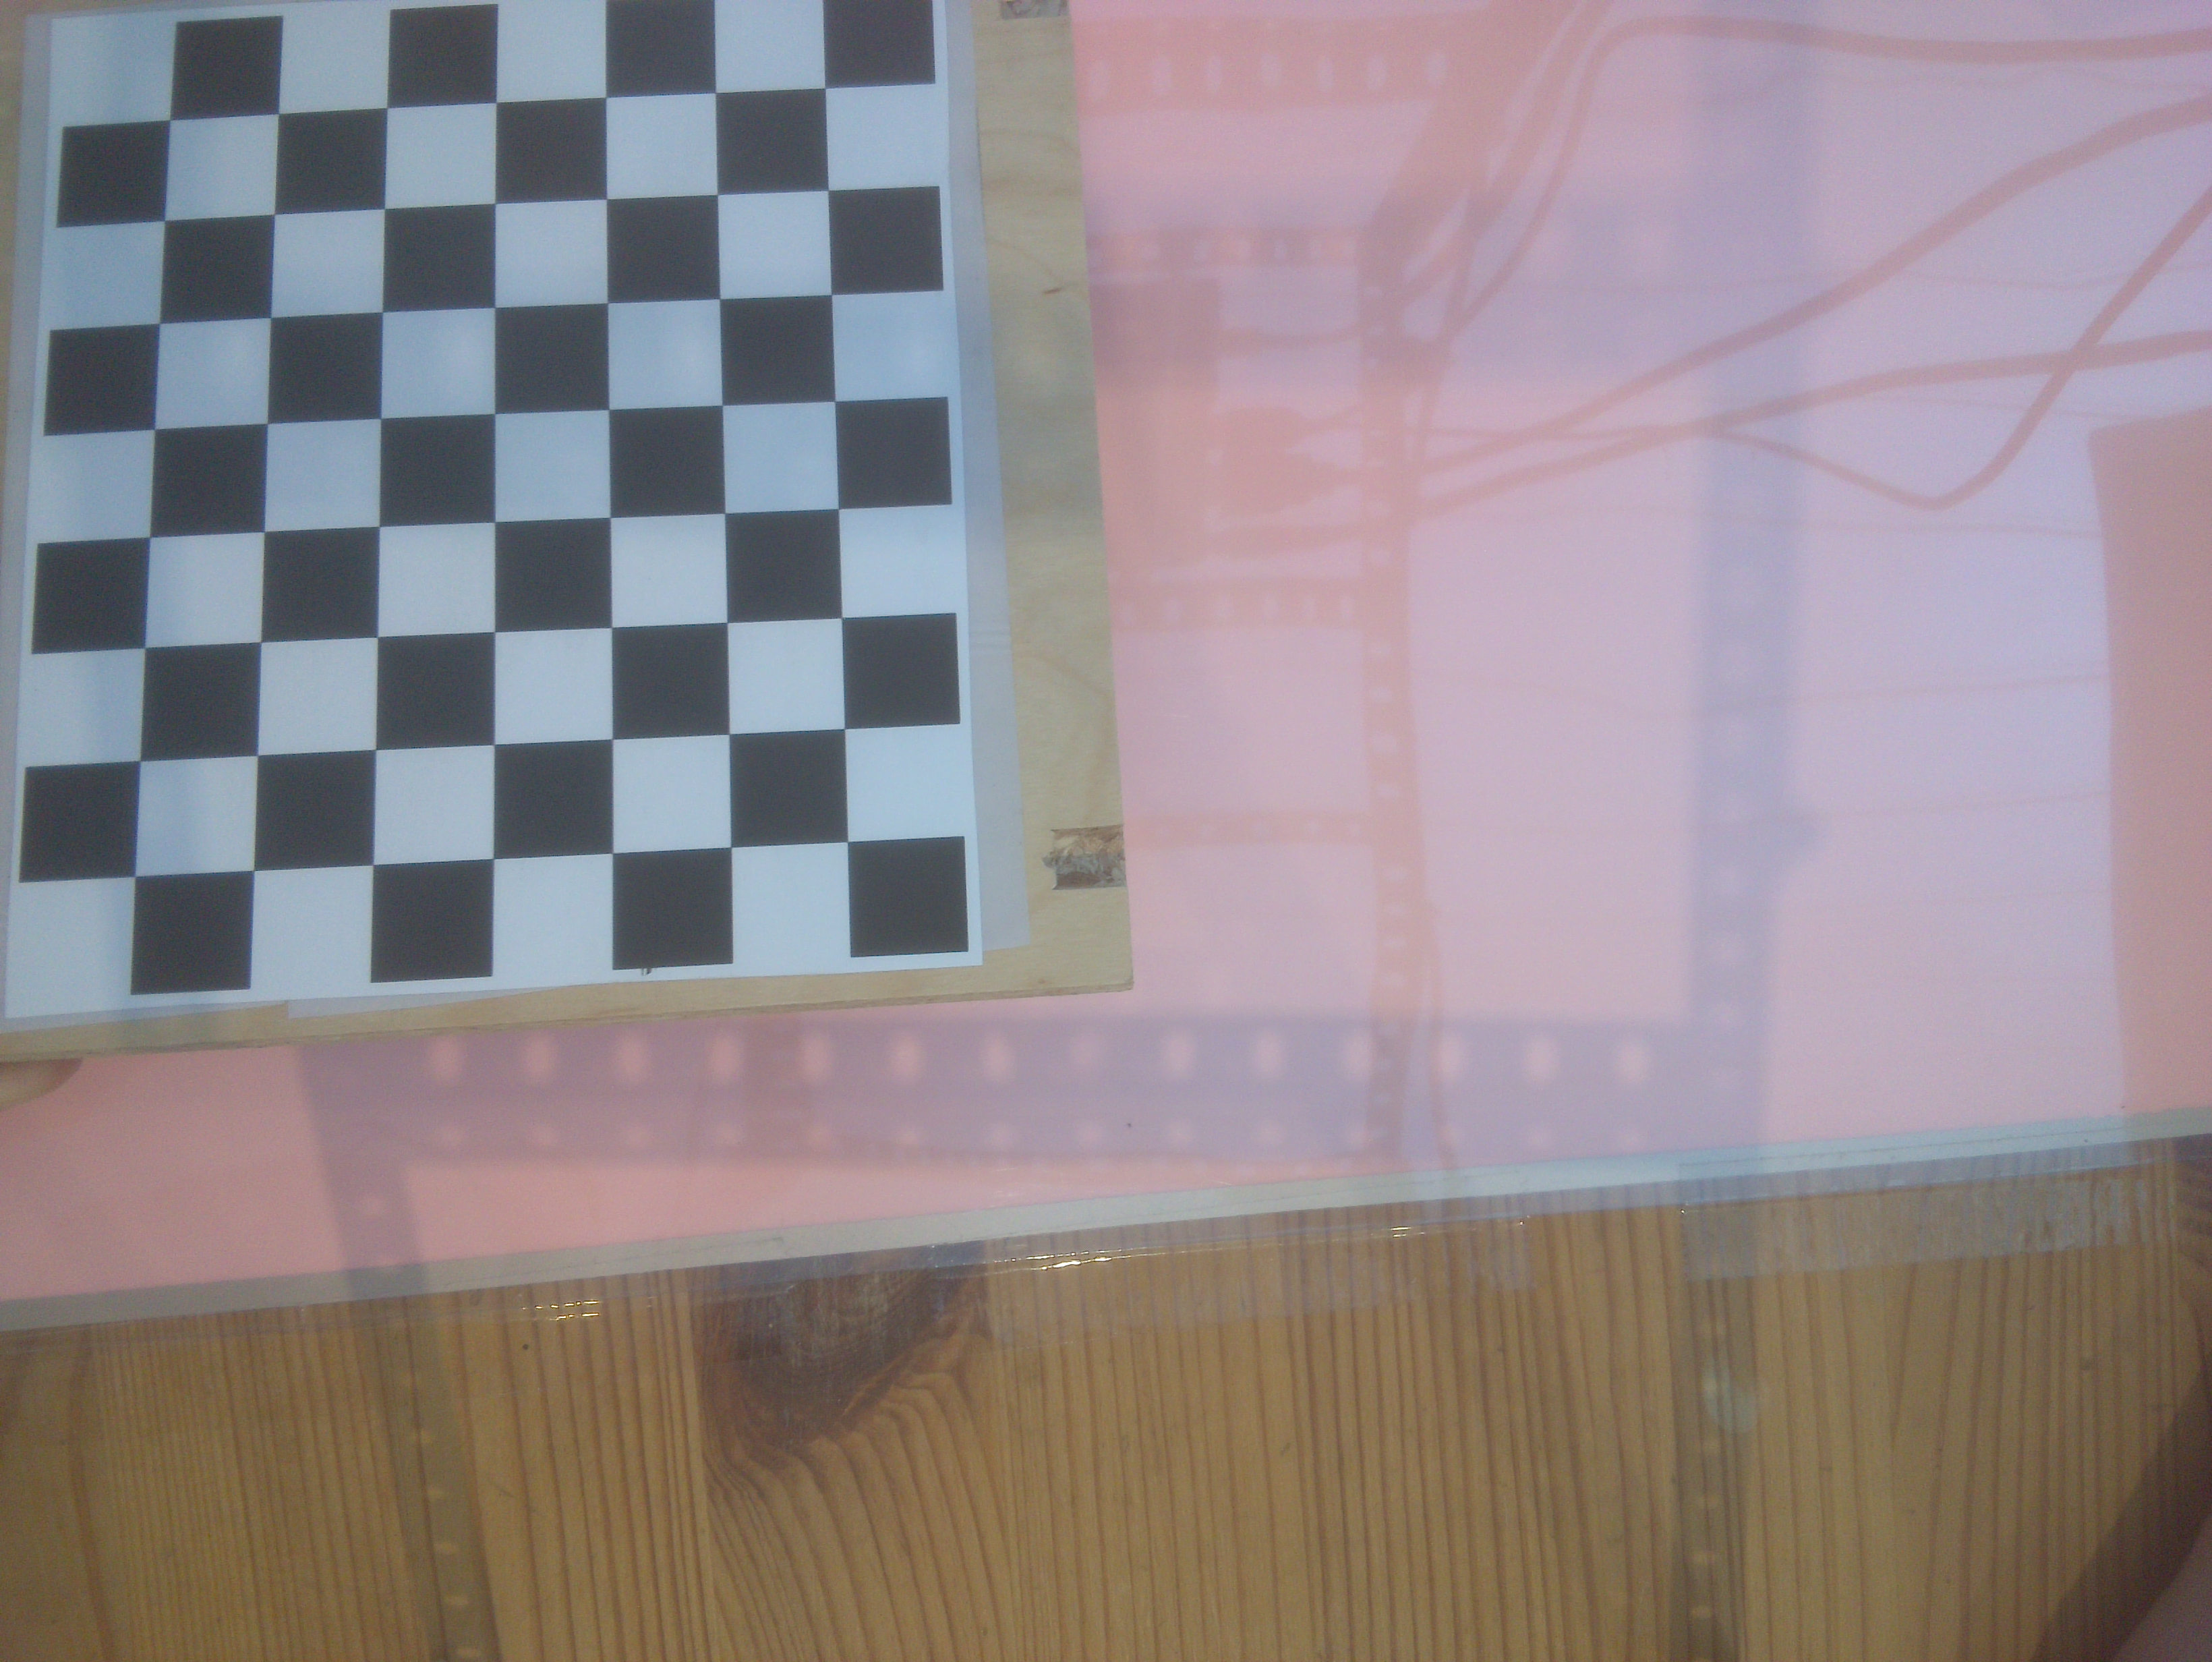
\includegraphics[width=0.3\linewidth]{3-development/calibration/images/im0.png}}
	\subfigure[\label{development:im1}]{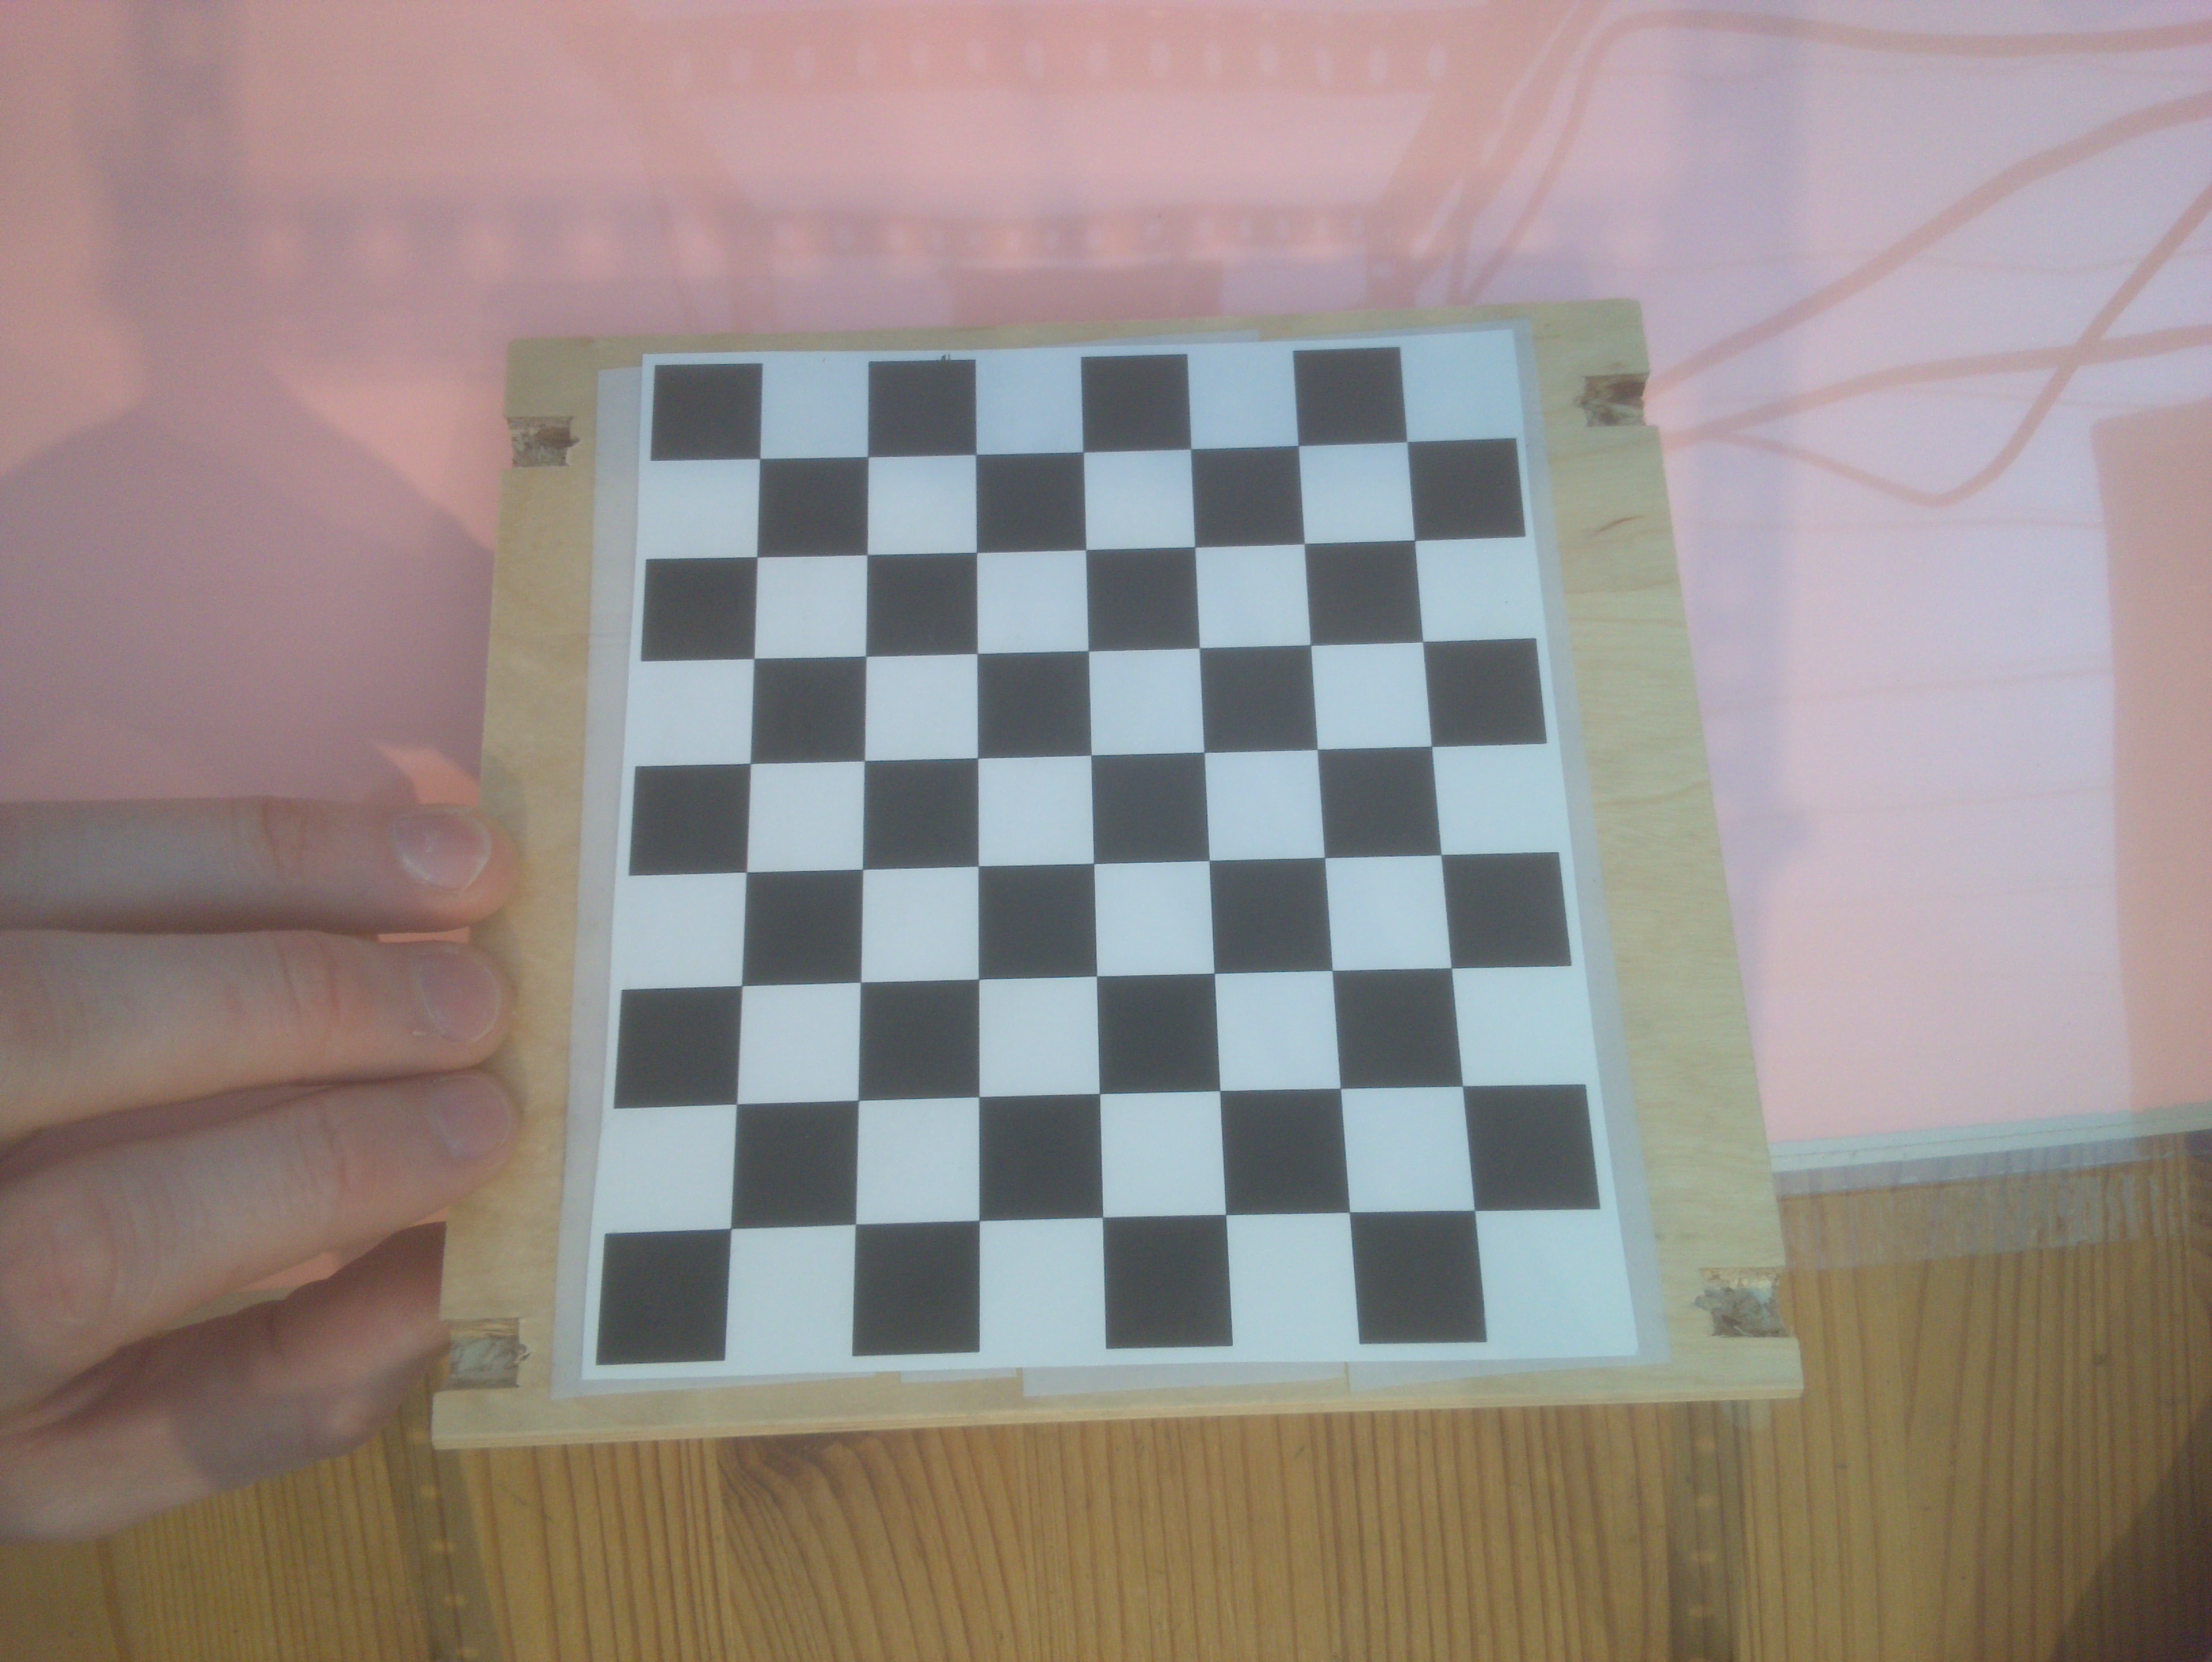
\includegraphics[width=0.3\linewidth]{3-development/calibration/images/im1.png}}
	\subfigure[\label{development:im2}]{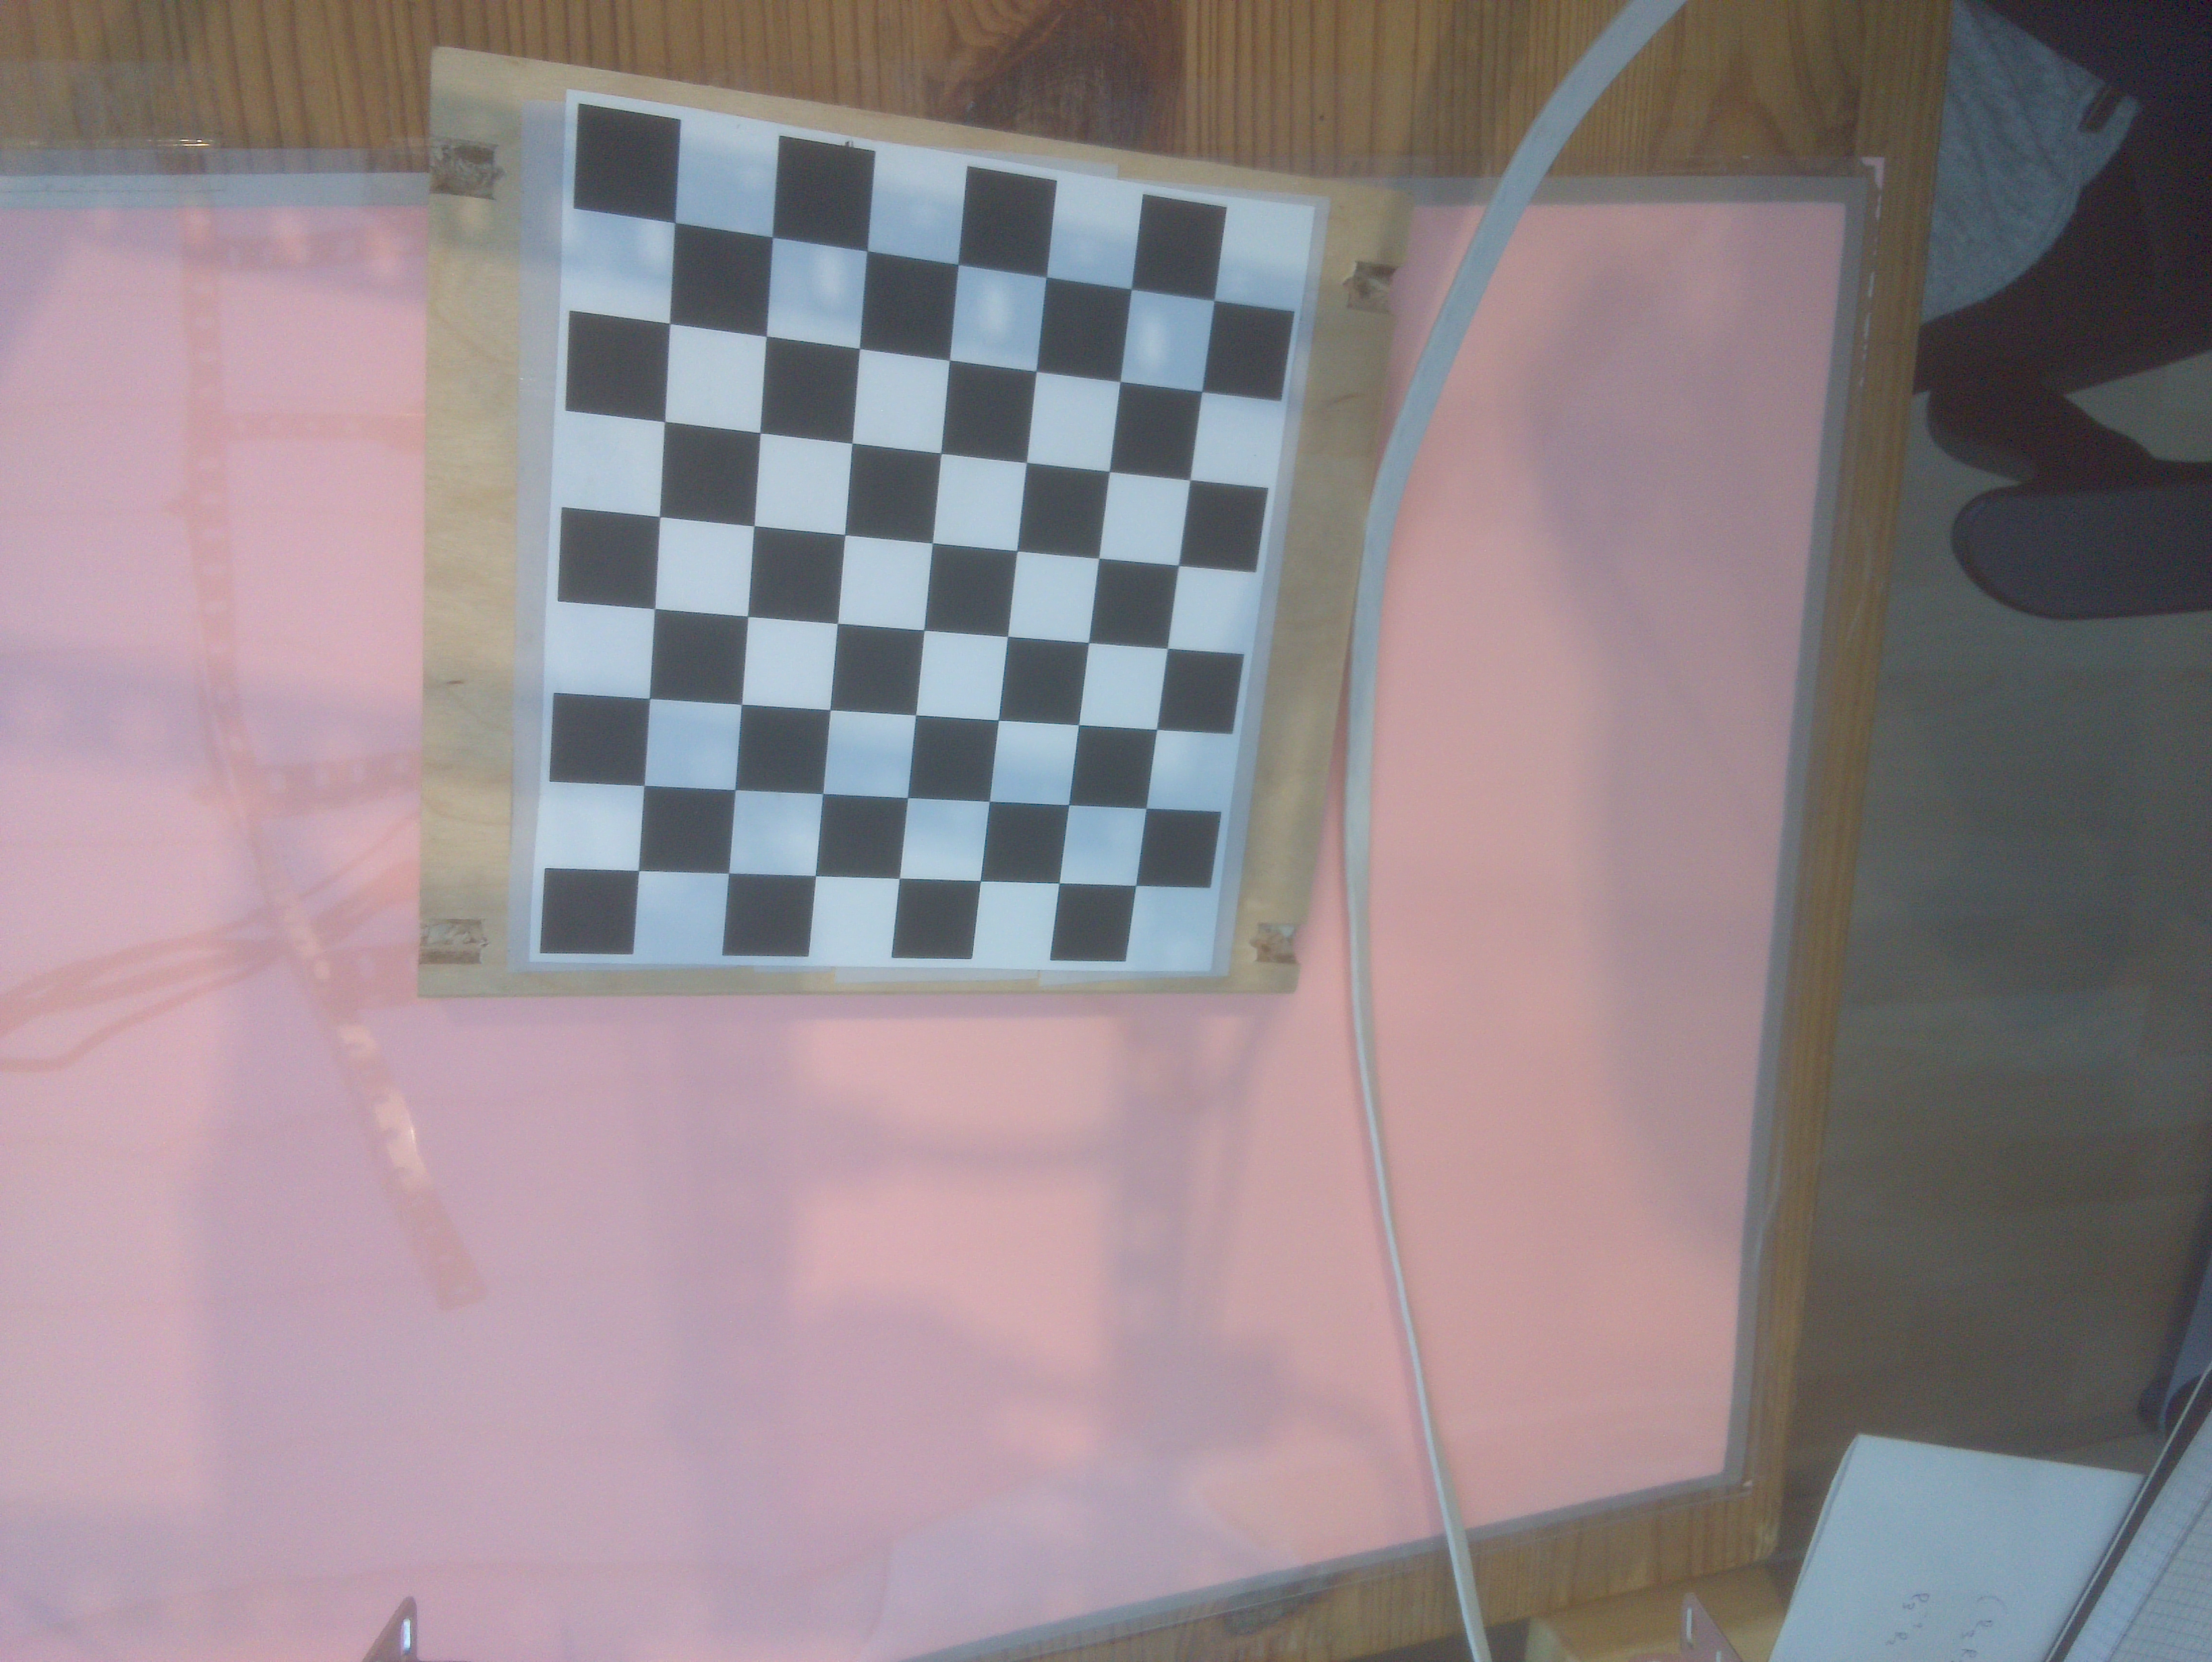
\includegraphics[width=0.3\linewidth]{3-development/calibration/images/im2.png}}
	
	\subfigure[\label{development:im3}]{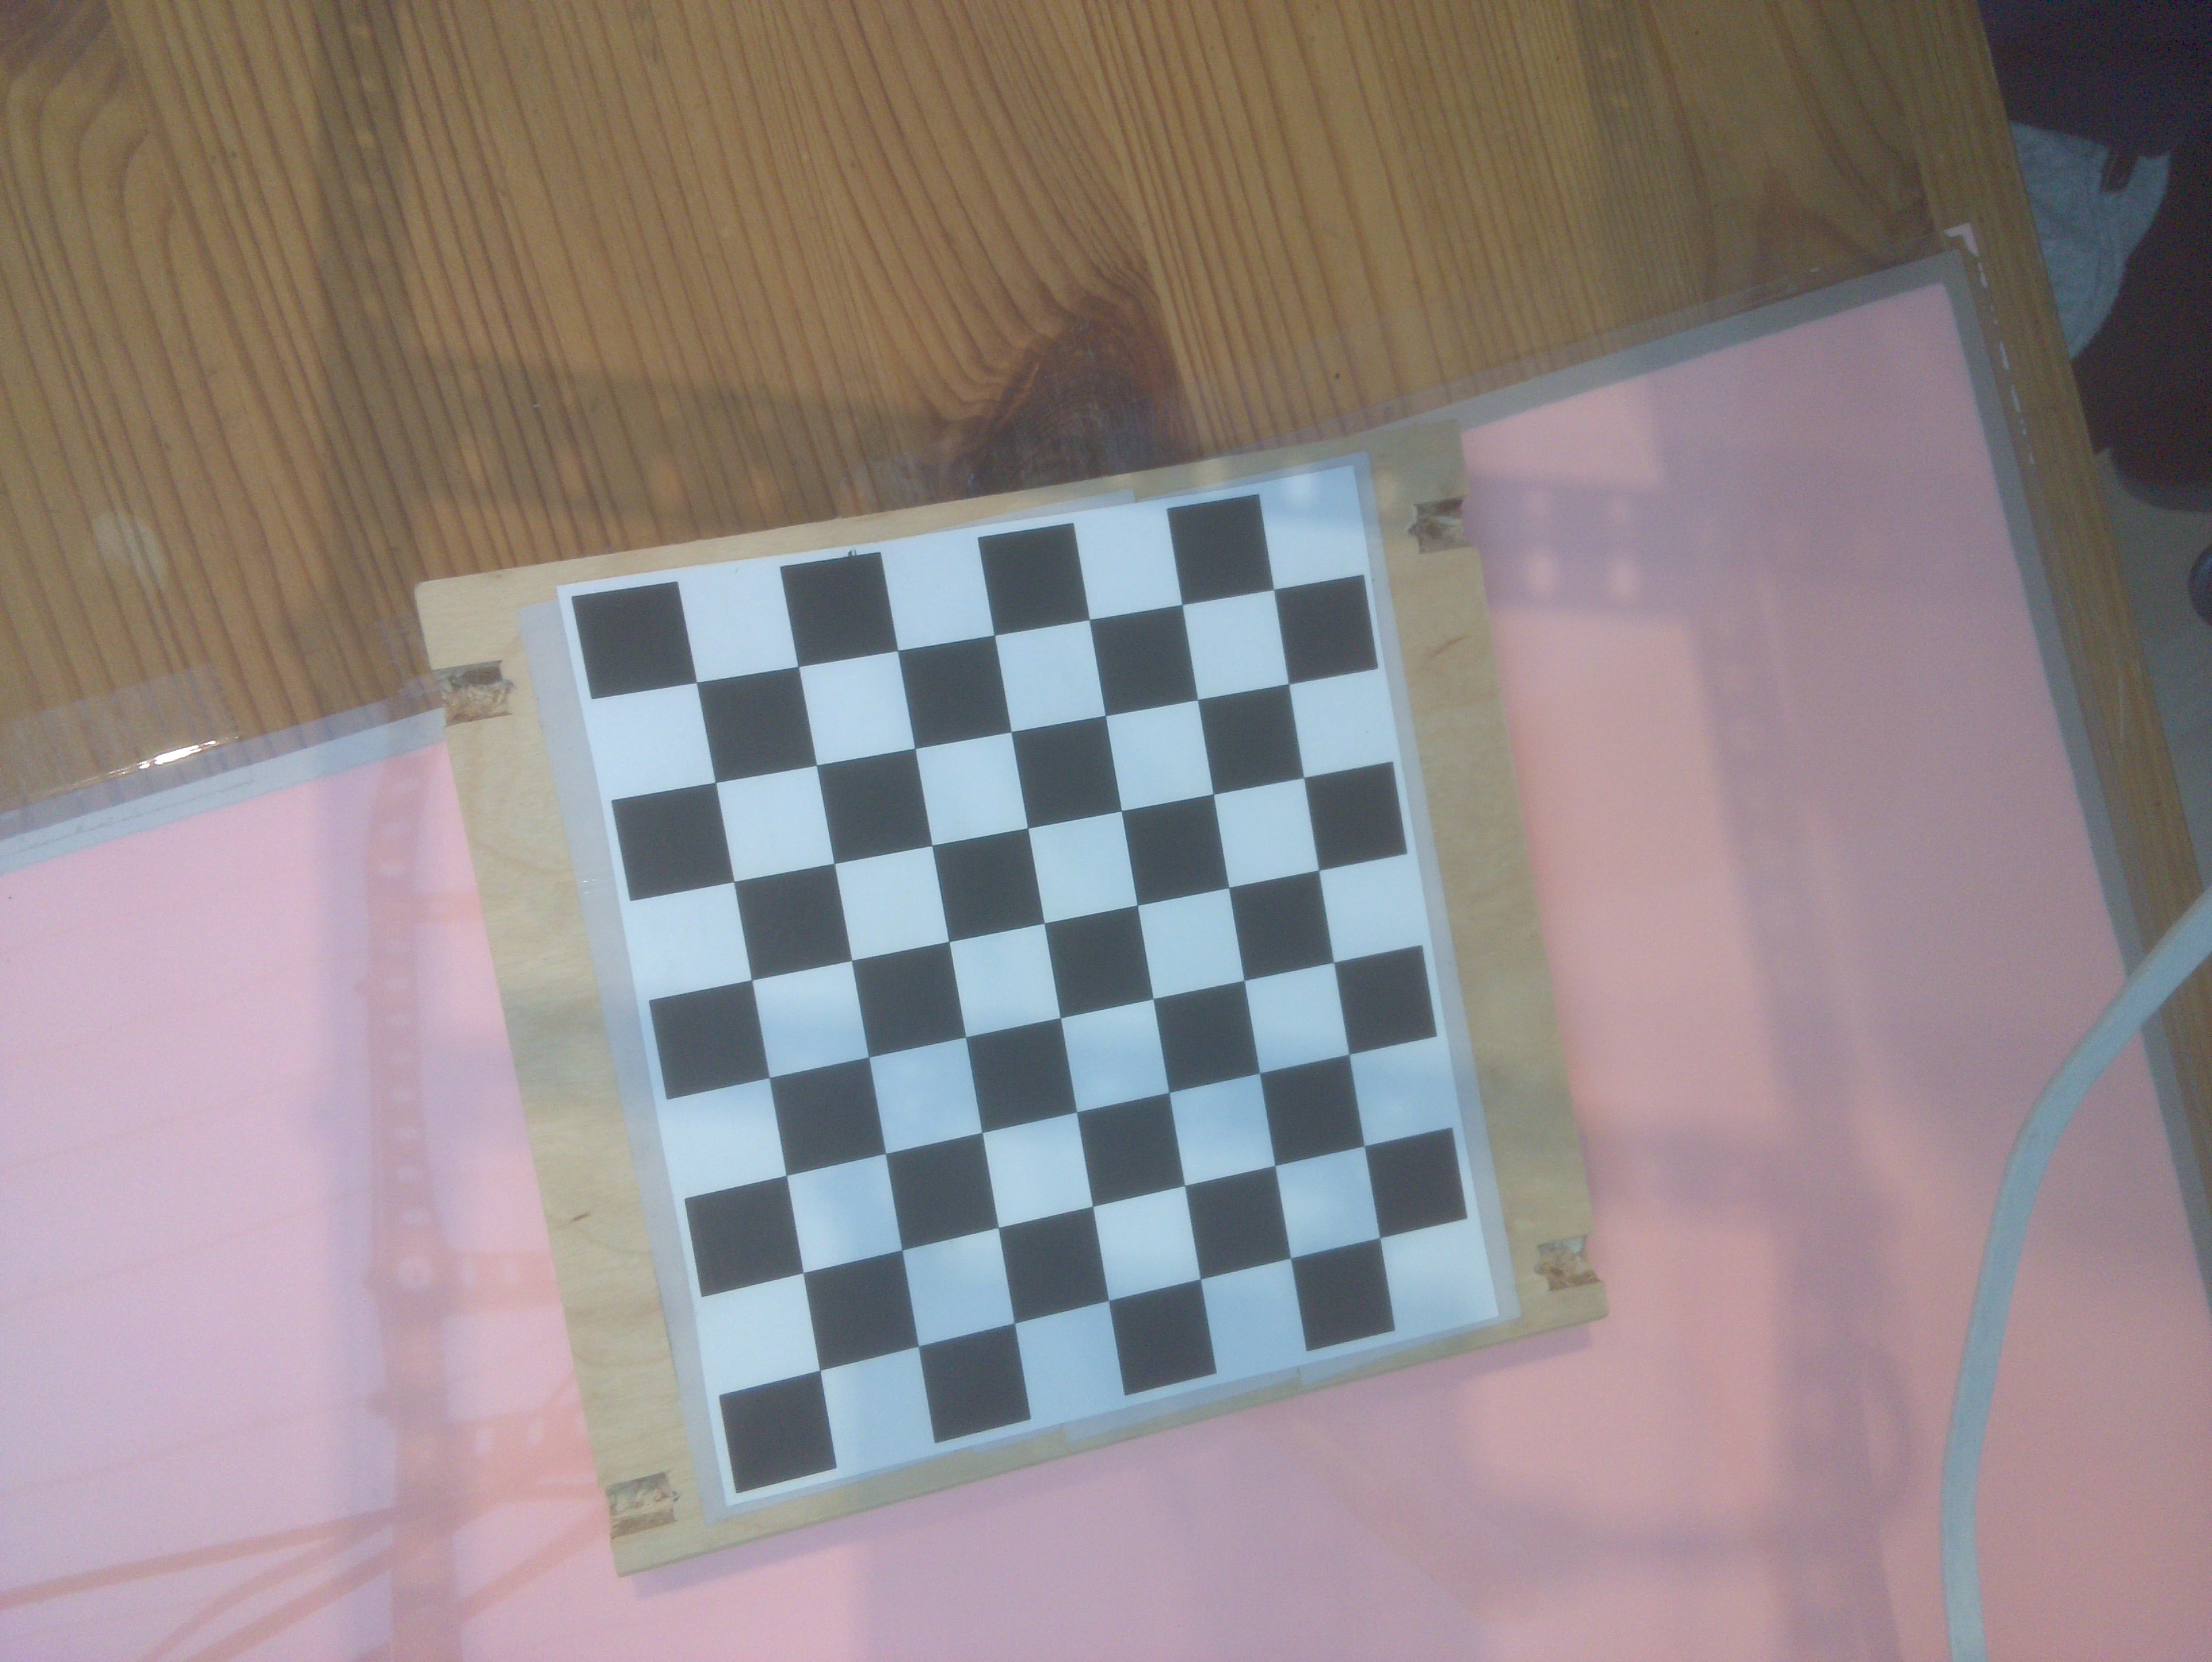
\includegraphics[width=0.3\linewidth]{3-development/calibration/images/im3.png}}
	\subfigure[\label{development:im4}]{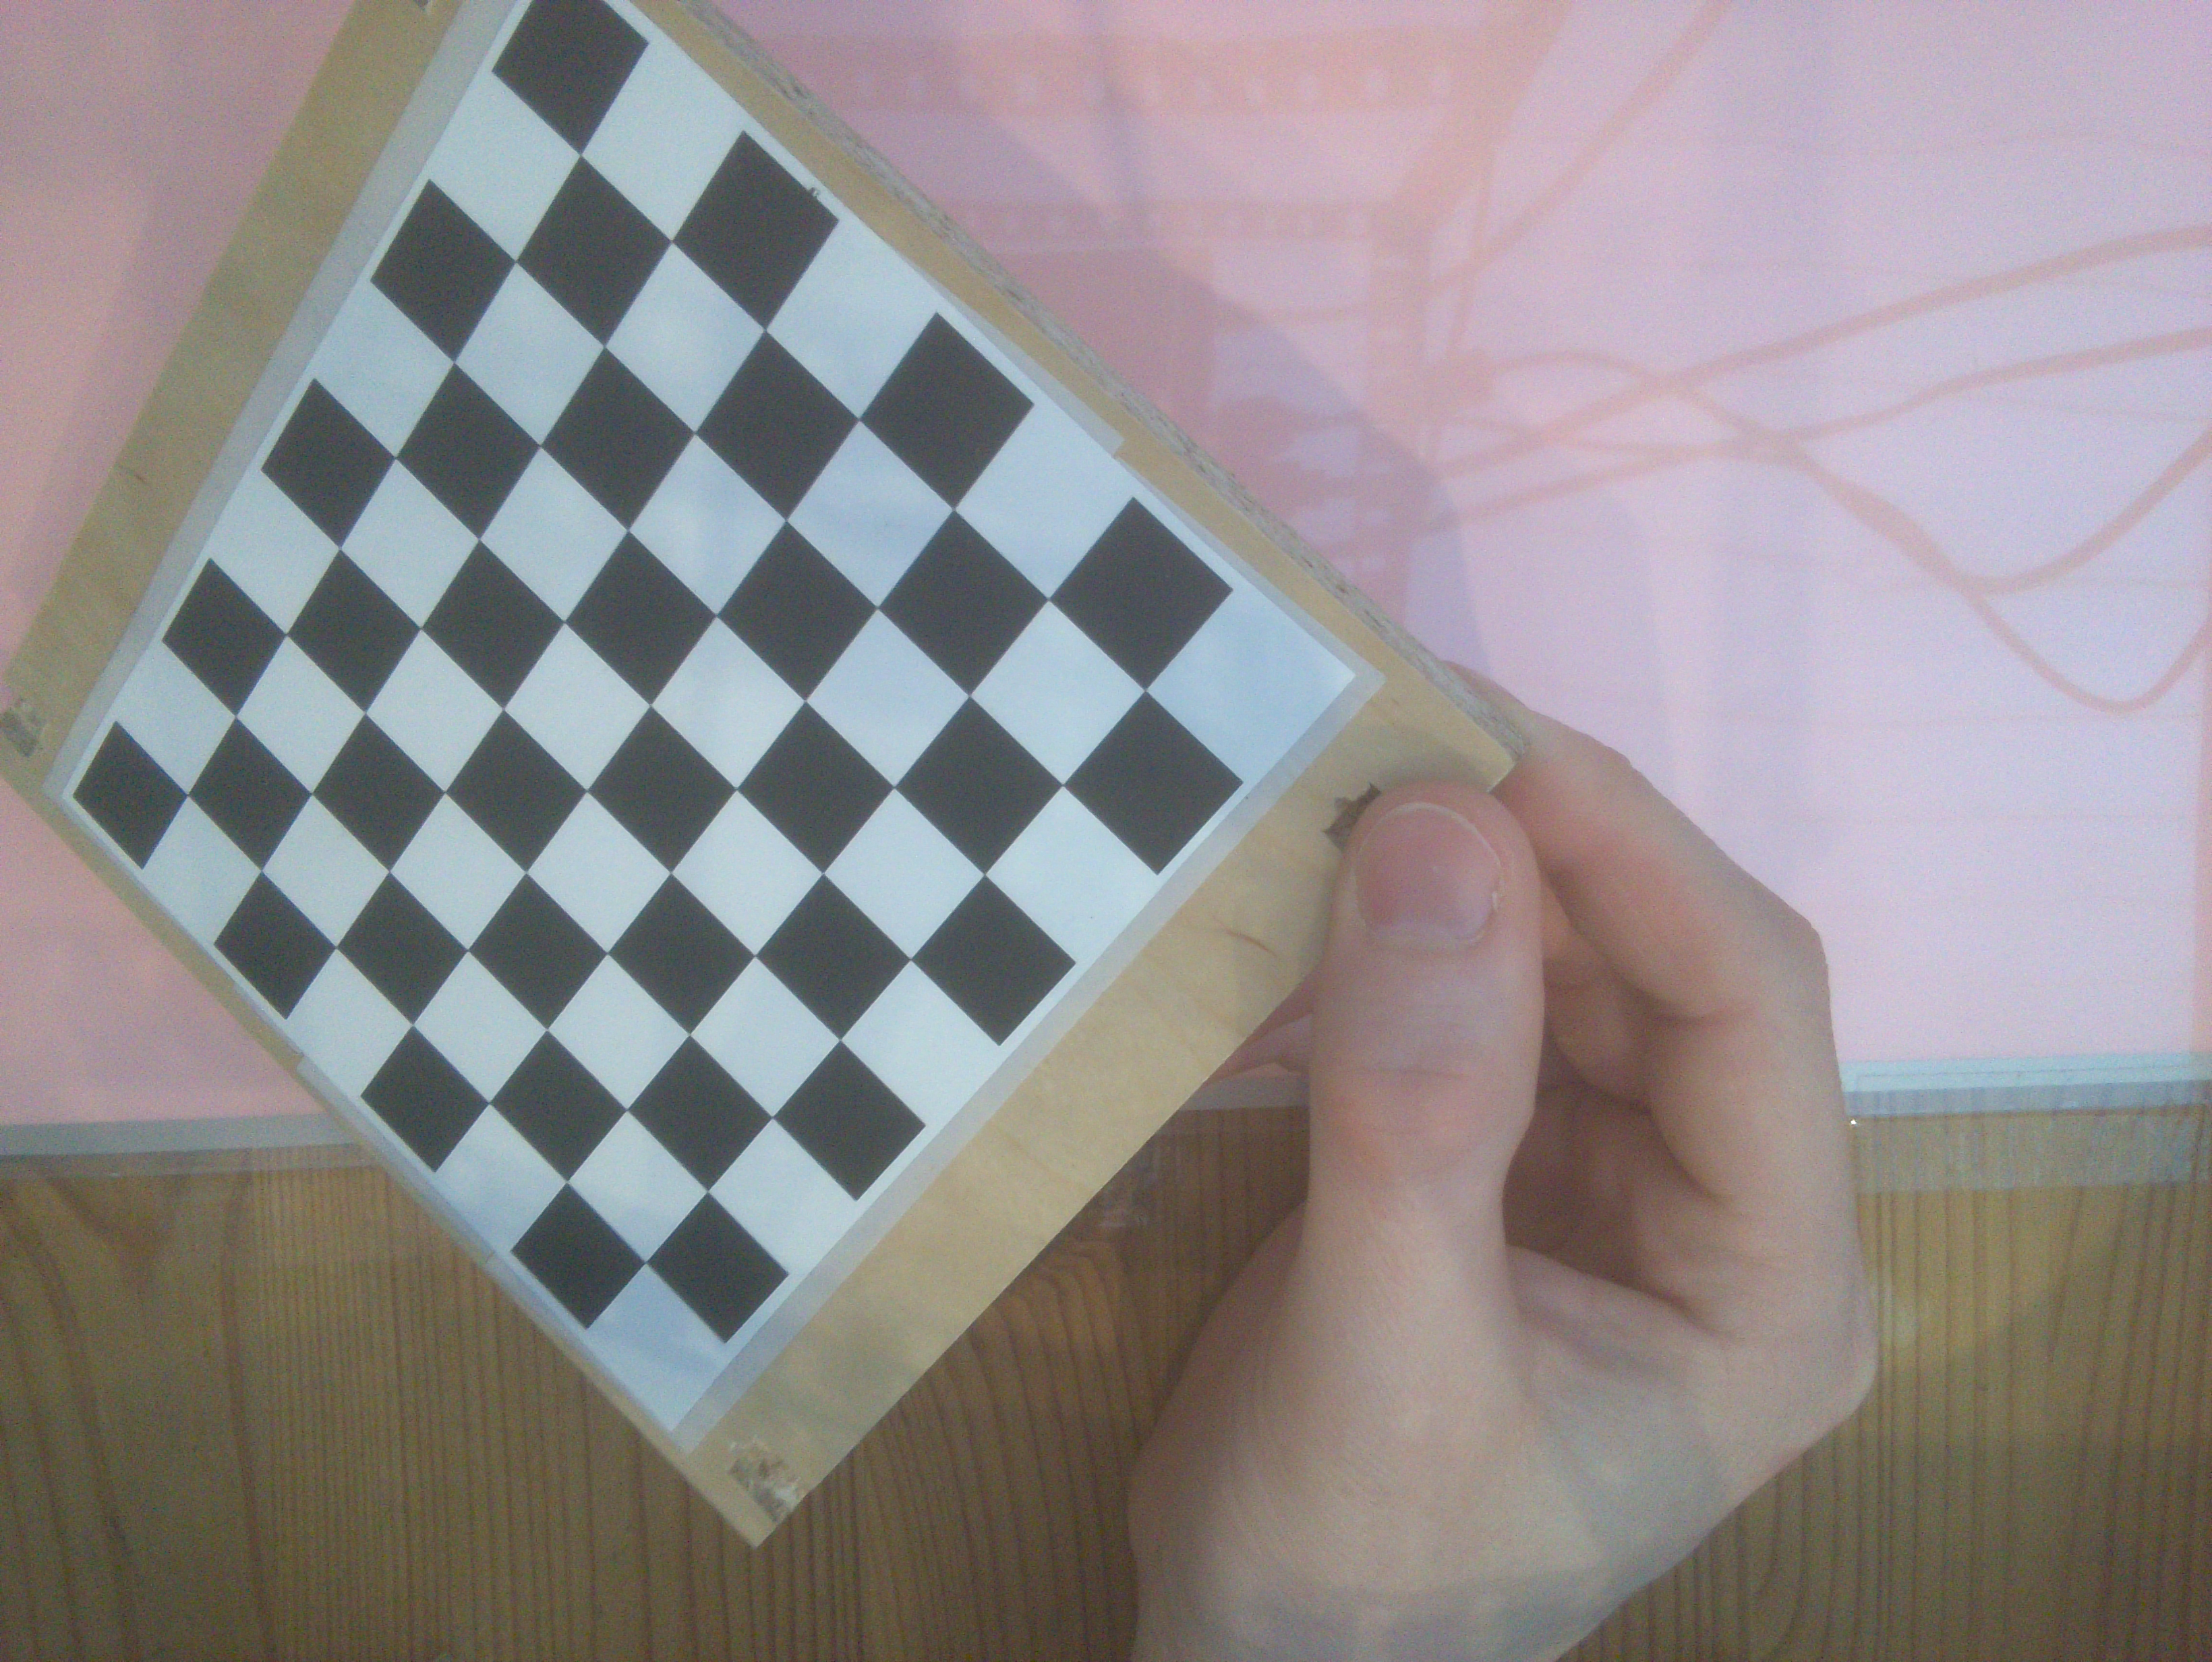
\includegraphics[width=0.3\linewidth]{3-development/calibration/images/im4.png}}
	\subfigure[\label{development:im5}]{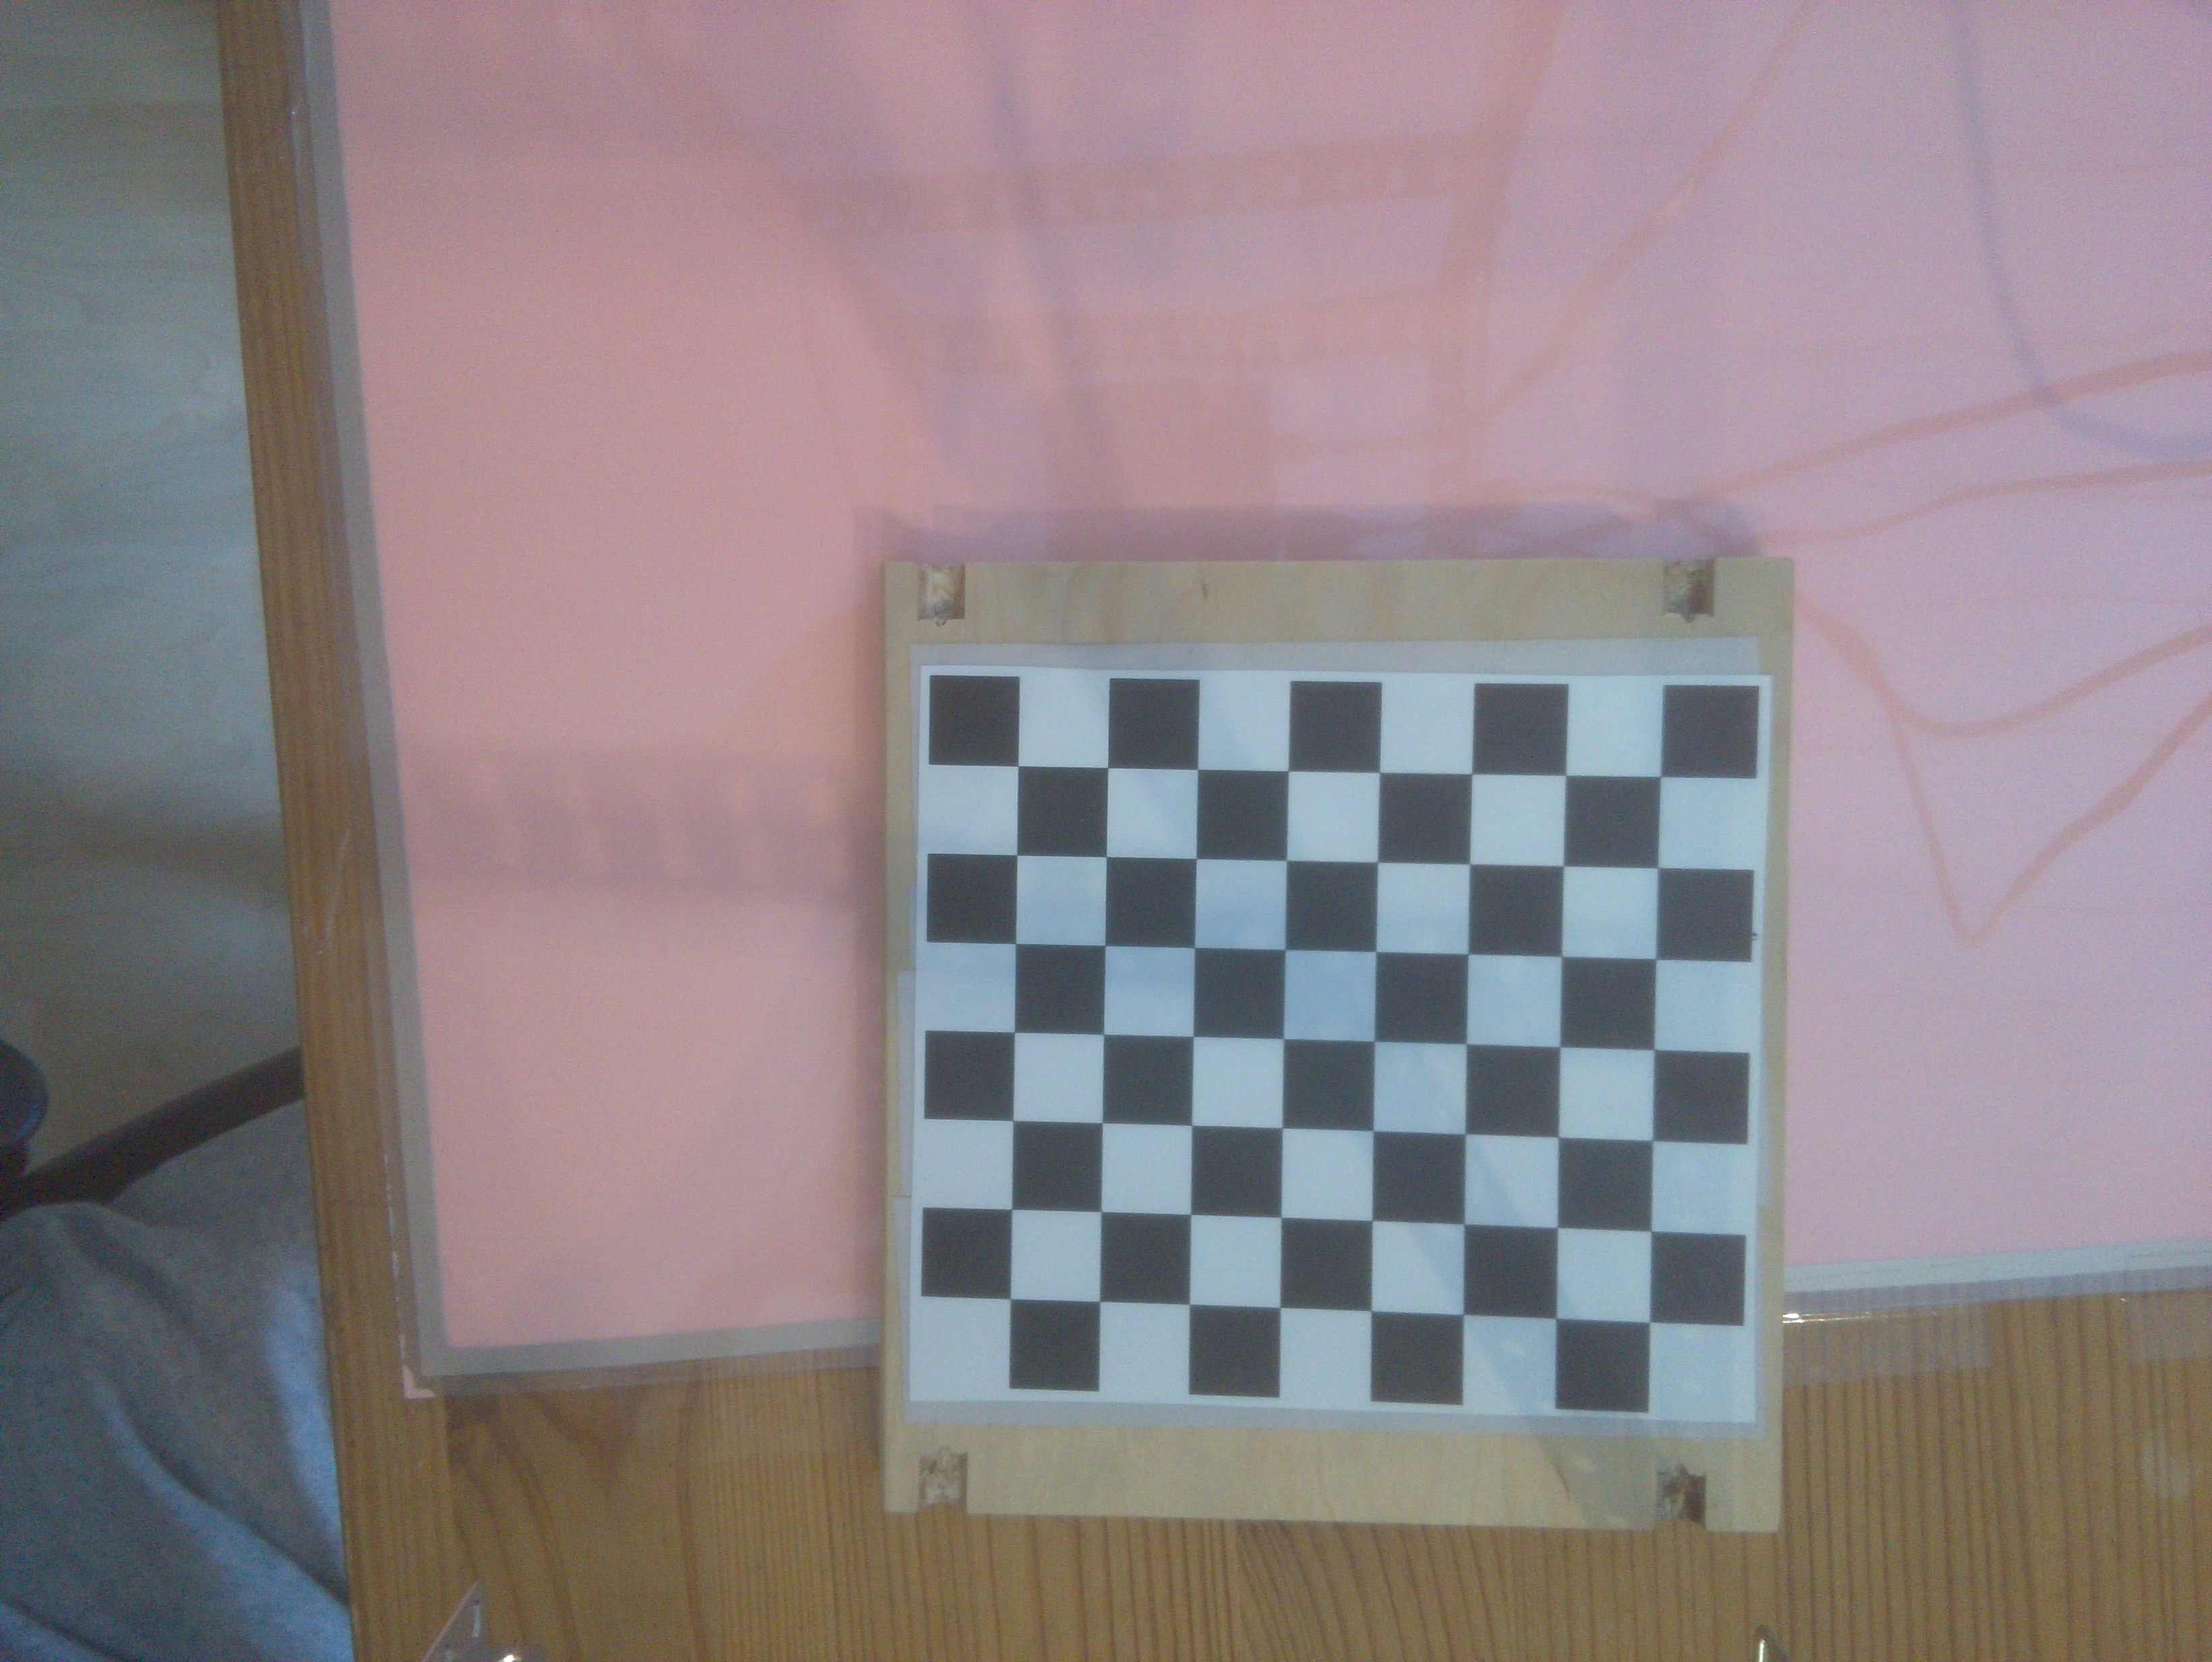
\includegraphics[width=0.3\linewidth]{3-development/calibration/images/im5.png}}
	\caption{Some of the 200 images \label{development:im}}		
\end{figure}

Randomly selected from these 200 are ten sets of each 20 images.
Now is the camera calibrated separately with each set.
To visualize the result, the difference from the distorted (real) and undistorted (corrected) on all locations of half the diagonal in the upper right quadrant of the image is plotted.
In other words, we take a look at the distortion between the image center and the upper right corner (min to max radius).
This plot is shown in Figure \ref{development:stat}.

\begin{figure}[ht]
	\centering
	\includegraphics[width=0.9\linewidth]{3-development/calibration/images/stat.pdf}
	\caption{Distortion over the radius according to different sets if images\label{development:stat}}
\end{figure}

The distortion model introduces decentering effects and one could argue, that this plot should be made in all quadrants of the image.
But since the decentering effects are rather small in comparison with the radial distortion which is symmetric with respect to the centerpoint it should be sufficient to plot only one quadrant.
it is therefore assumed, that if the distortions are high in one quadrant, that the distortions in all other quadrants is also high and vice versa.



